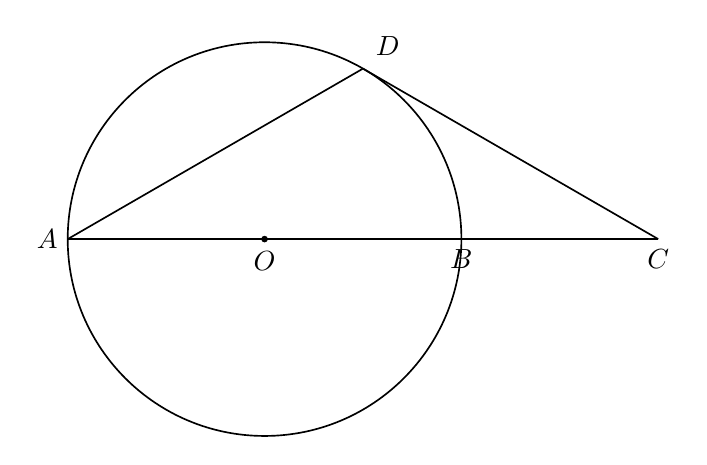
\begin{tikzpicture}[x=1cm,y=1cm,line width=.6pt,font=\normalsize]
\coordinate (O) at (0,0);
\coordinate (A) at (-2.5,0);
\coordinate (B) at (2.5,0);
\coordinate (C) at (5,0);
\coordinate (D) at (1.25,2.1651);
\draw[black] (O) circle[radius=2.5cm];
\draw[black] (A)--(C);
\draw[black] (A)--(D);
\draw[black] (D)--(C);
\fill[black] (O) circle[radius=1.2pt];
\node[left] at (A) {$A$};
\node[below, yshift=-1pt] at (O) {$O$};
\node[below] at (B) {$B$};
\node[below] at (C) {$C$};
\node[above right, xshift=1pt, yshift=1pt] at (D) {$D$};
\end{tikzpicture}
